\section{Experimental Results}
\label{sec:results}

This section presents the quantitative findings of our empirical study across $N=500$ requirements. All statistical significance tests were evaluated at $\alpha = 0.05$.

\subsection{RQ1: Semantic Similarity}
RQ1 investigates which prompting technique achieves the highest semantic similarity compared with the Ground Truth scenarios.

Table~\ref{tab:rq1_results} presents the mean Cosine Similarity, threshold, $p$-value (One-Sample Wilcoxon Signed-Rank Test), Cohen's $d$ effect size, and baseline evaluation status across $N=500$ requirements. Figure~\ref{fig:distribution} illustrates the score distribution across the three prompting techniques.

\begin{table}[htbp]
\caption{RQ1: SBERT Cosine Similarity Results ($N=500$)}
\label{tab:rq1_results}
\begin{center}
\resizebox{\columnwidth}{!}{%
\begin{tabular}{lccccc}
\hline
\textbf{Technique} & \textbf{Mean Sim.} & \textbf{Threshold} & \textbf{p-value} & \textbf{Effect Size ($d$)} & \textbf{Status} \\
\hline
Zero-Shot & 0.8088 & 0.80 & 0.0000 & 0.0827 & \textbf{Pass} \\
Few-Shot & 0.8218 & 0.80 & 0.0007 & 0.2038 & \textbf{Pass} \\
CoT & 0.8168 & 0.80 & 0.0000 & 0.1644 & \textbf{Pass} \\
\hline
\end{tabular}%
}
\end{center}
\end{table}

\begin{figure}[htbp]
    \centering
    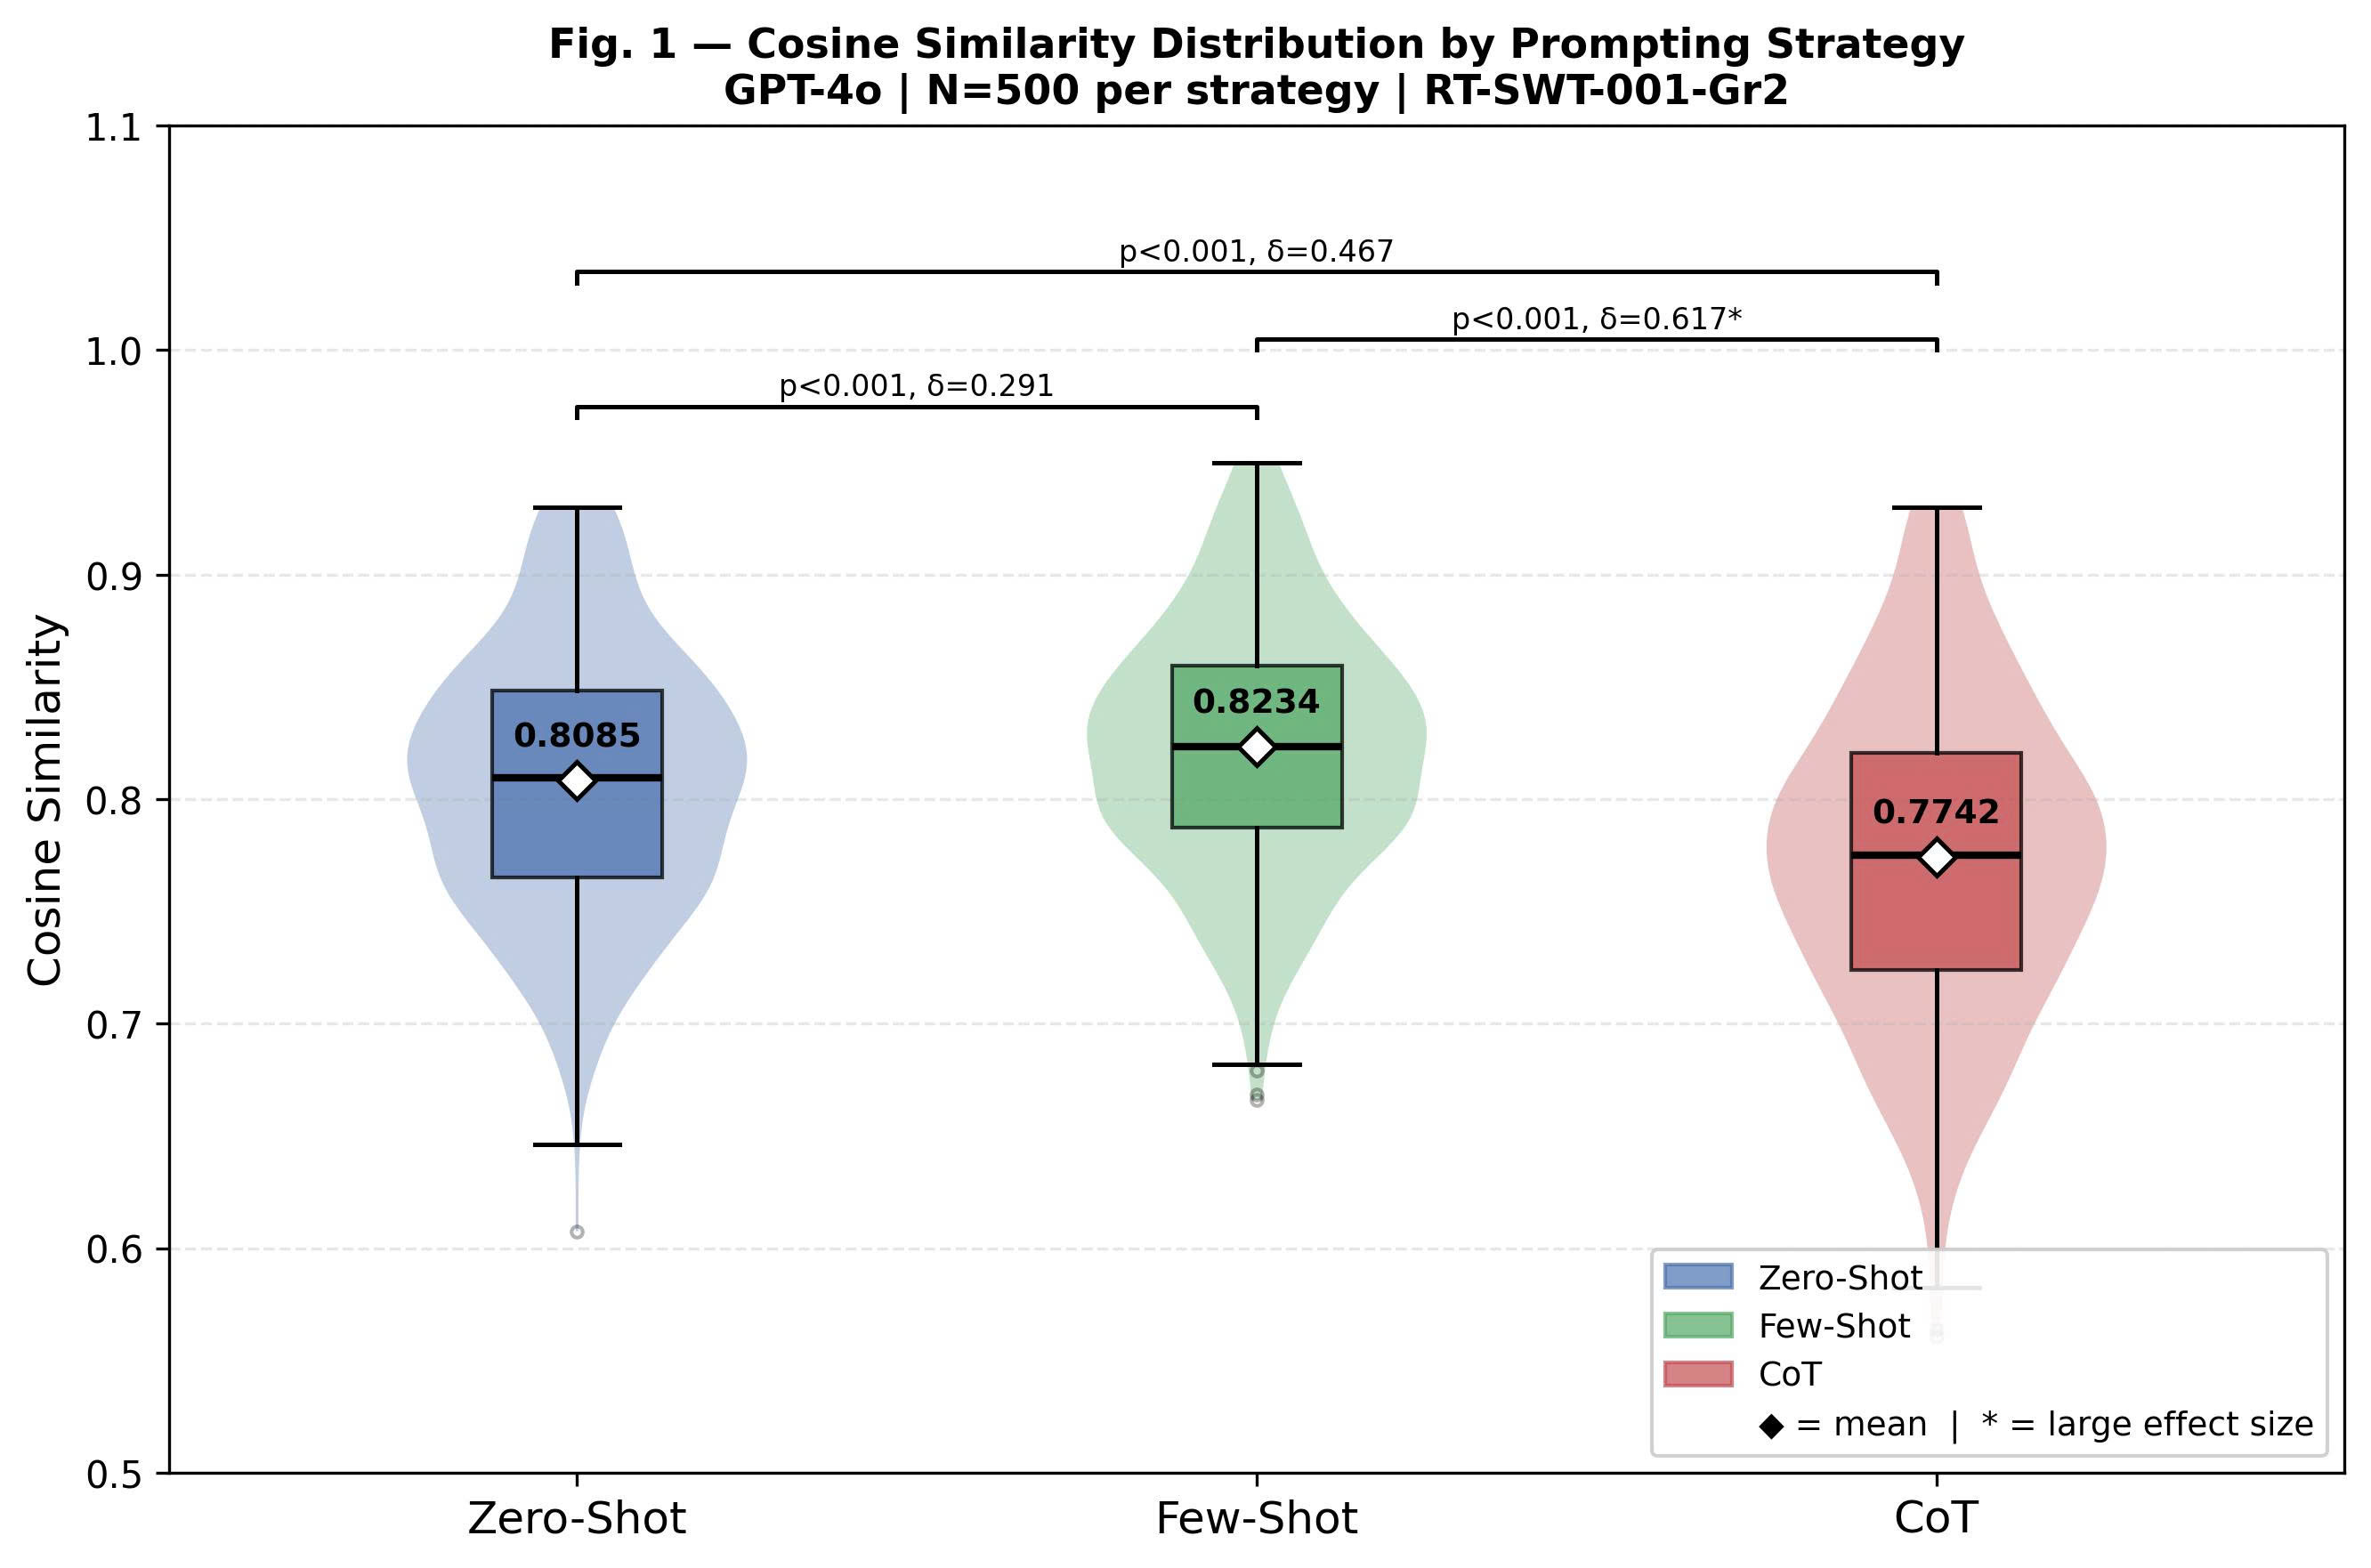
\includegraphics[width=\columnwidth]{figures/fig1_distribution.png}
    \caption{Semantic Similarity (SBERT Cosine) distribution across Zero-Shot, Few-Shot, and Chain-of-Thought prompting techniques ($N=500$).}
    \label{fig:distribution}
\end{figure}

Few-Shot prompting achieved the highest average semantic similarity of $0.8218$ ($p = 0.0007, d = 0.2038$, Pass). Chain-of-Thought prompting achieved a mean Cosine Similarity of $0.8168$ ($p = 0.0000, d = 0.1644$, Pass). Zero-Shot prompting achieved a mean Cosine Similarity of $0.8088$ ($p = 0.0000, d = 0.0827$, Pass).

\textit{Conclusion for RQ1:} Few-Shot prompting achieves the highest semantic similarity compared with the Ground Truth scenarios, with all three techniques exceeding the $0.80$ threshold ($p < 0.001$).

\subsection{RQ2: Executable Syntax Validity}
RQ2 investigates which prompting technique produces the highest executable syntax validity.

Table~\ref{tab:rq2_results} reports the Gherkin keyword validation, Python AST parse rate, baseline threshold, $p$-value (One-Sample Binomial Exact Test), and status across $N=500$ requirements. Figure~\ref{fig:comparison} displays the comparative parse rates. Table~\ref{tab:content_stats} presents structural content statistics.

\begin{table}[htbp]
\caption{RQ2: Gherkin Syntax and Python AST Parse Rate Results ($N=500$)}
\label{tab:rq2_results}
\begin{center}
\resizebox{\columnwidth}{!}{%
\begin{tabular}{lccccc}
\hline
\textbf{Technique} & \textbf{Gherkin Valid} & \textbf{AST Parse Rate} & \textbf{Threshold} & \textbf{p-value} & \textbf{Status} \\
\hline
Zero-Shot & 500/500 (100.0\%) & 499/500 (99.8\%) & 85\% & 0.0000 & \textbf{Pass} \\
Few-Shot & 496/500 (99.2\%) & 500/500 (100.0\%) & 85\% & 0.0000 & \textbf{Pass} \\
CoT & 500/500 (100.0\%) & 500/500 (100.0\%) & 85\% & 0.0000 & \textbf{Pass} \\
\hline
\end{tabular}%
}
\end{center}
\end{table}

\begin{figure}[htbp]
    \centering
    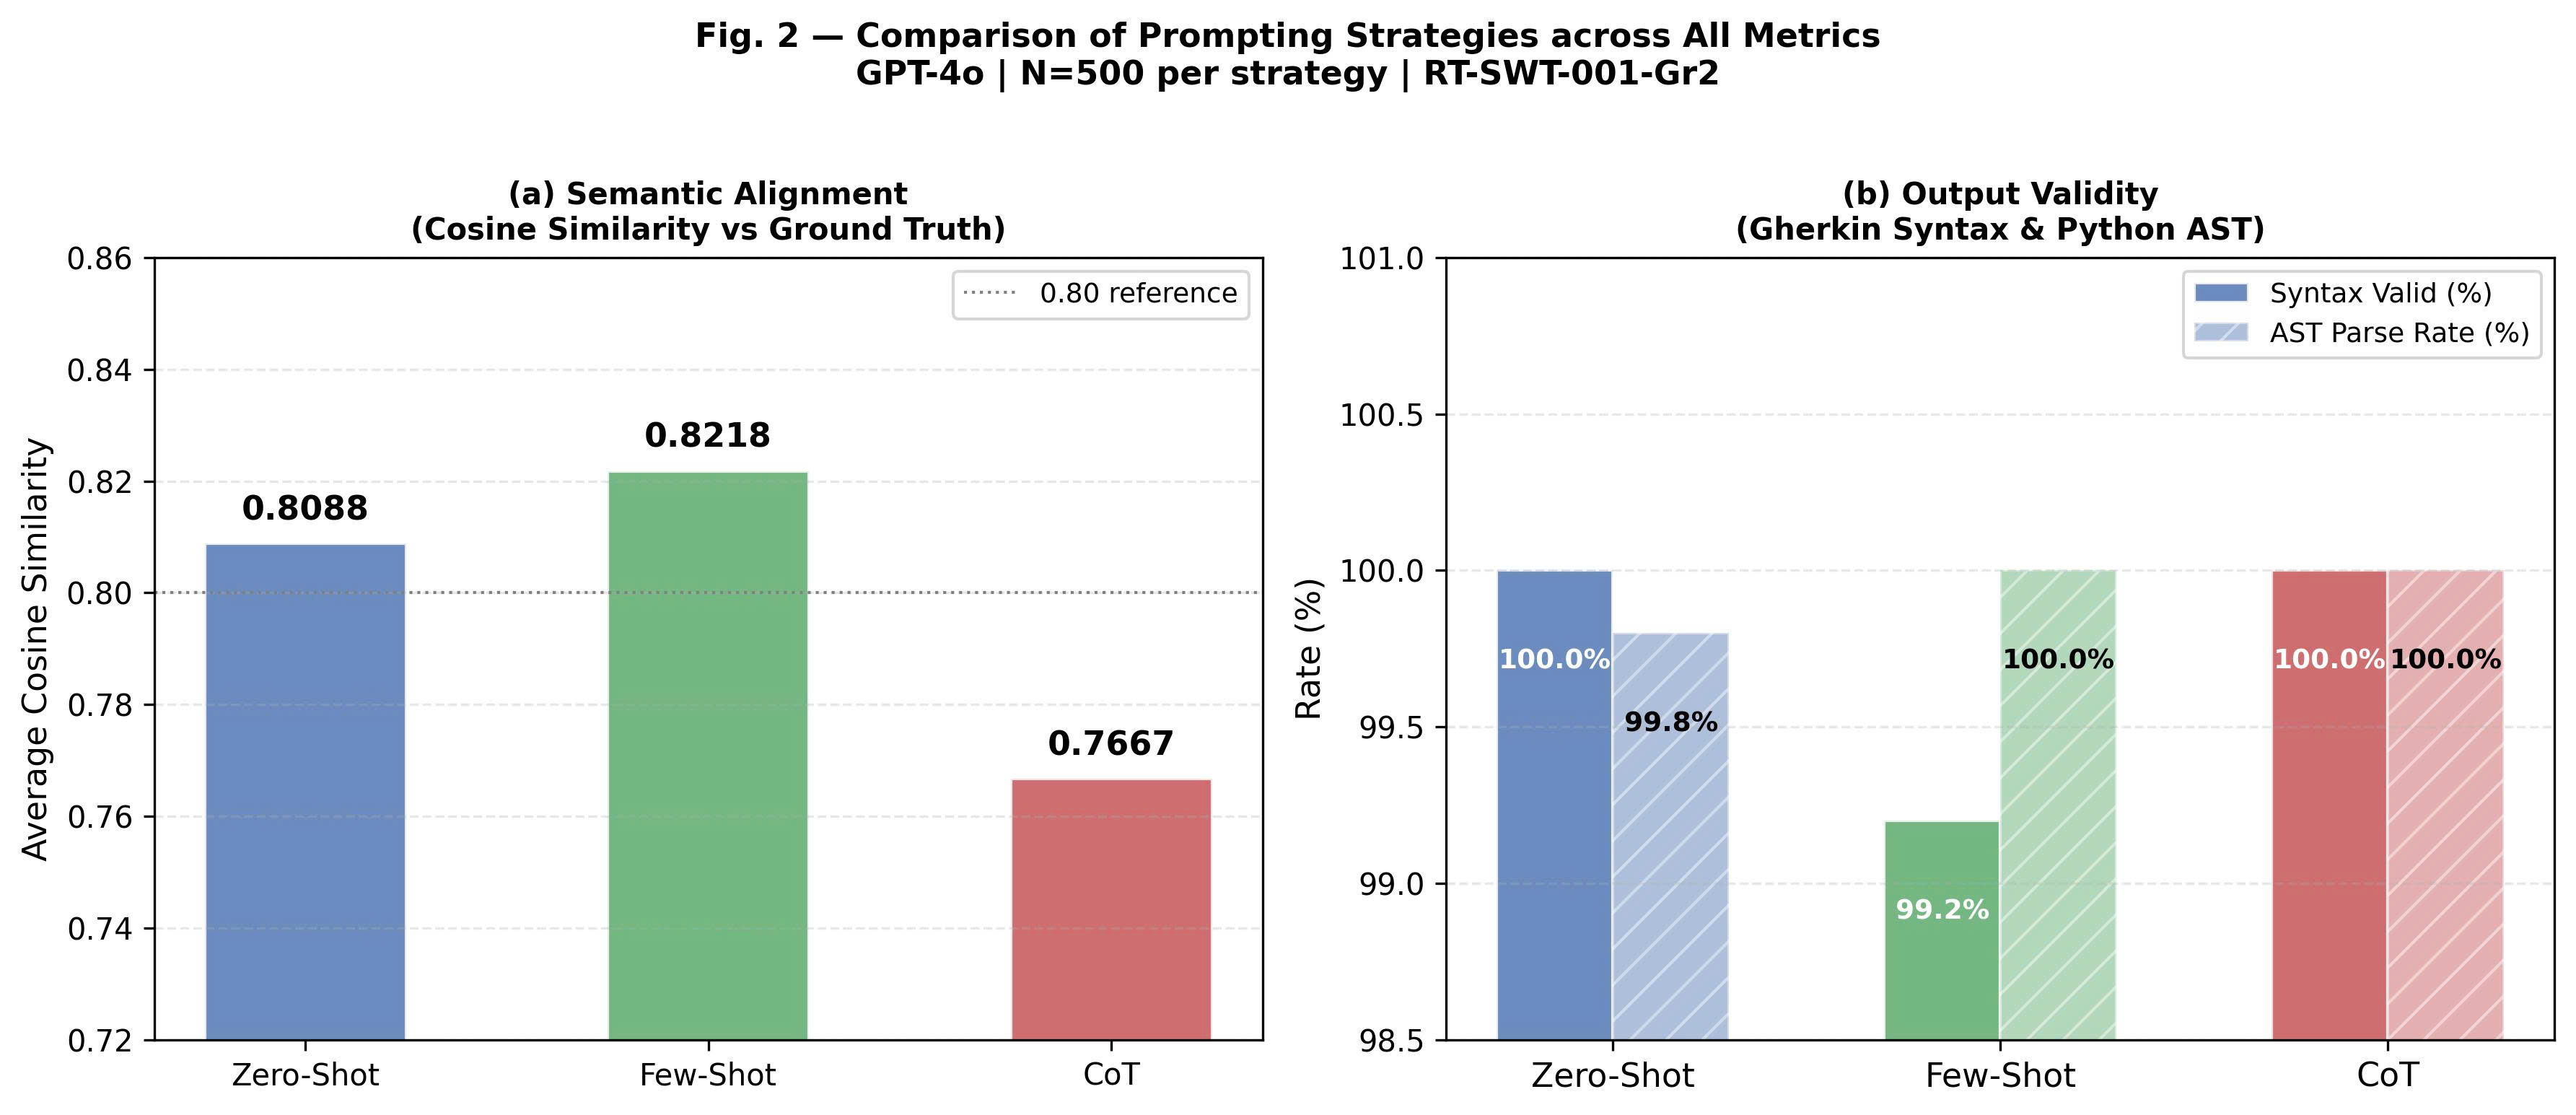
\includegraphics[width=0.85\columnwidth]{figures/fig2_comparison.png}
    \caption{Executable Syntax Rate (AST Parse) comparison across prompting techniques ($N=500$).}
    \label{fig:comparison}
\end{figure}

\begin{table}[htbp]
\caption{Structural Content Statistics across Prompting Techniques}
\label{tab:content_stats}
\begin{center}
\resizebox{\columnwidth}{!}{%
\begin{tabular}{lcccccc}
\hline
\textbf{Technique} & \textbf{Avg Steps} & \textbf{Avg Scenarios} & \textbf{Has And (\%)} & \textbf{Avg Words} & \textbf{Avg Lines} & \textbf{Step Bounds} \\
\hline
Zero-Shot & 4.35 & 1.00 & 65.8\% & 128.9 & 30.2 & [3, 11] \\
Few-Shot & 5.26 & 1.34 & 65.4\% & 128.5 & 32.4 & [2, 23] \\
CoT & 5.17 & 1.00 & 98.6\% & 132.5 & 35.9 & [3, 15] \\
\hline
\end{tabular}%
}
\end{center}
\end{table}

Few-Shot and CoT prompting achieved a perfect $100.0\%$ Python AST parse rate (500/500, $p = 0.0000$), while Zero-Shot achieved $99.8\%$ (499/500, $p = 0.0000$). For Gherkin structural syntax, Zero-Shot and CoT achieved $100.0\%$ (500/500), while Few-Shot achieved $99.2\%$ (496/500).

\textit{Conclusion for RQ2:} Few-Shot and Chain-of-Thought prompting produce the highest executable AST syntax validity ($100.0\%$), with all techniques significantly exceeding the $85\%$ benchmark ($p < 0.001$).

\subsection{RQ3: Comparative Effectiveness}
RQ3 investigates whether there are statistically significant differences among the prompting techniques.

Table~\ref{tab:rq3_pairwise} summarizes the Pairwise Wilcoxon Signed-Rank test statistics, $p$-values, decision outcomes, and Cohen's $d$ effect sizes for semantic similarity comparisons across $N=500$ requirements. Paired McNemar tests for AST syntactic validity yielded $p = 1.0000$ across all pairwise comparisons.

\begin{table}[htbp]
\caption{RQ3: Pairwise Wilcoxon Signed-Rank Test Results and Effect Sizes}
\label{tab:rq3_pairwise}
\begin{center}
\resizebox{\columnwidth}{!}{%
\begin{tabular}{lcccc}
\hline
\textbf{Comparison Pair} & \textbf{Statistic ($W$)} & \textbf{p-value} & \textbf{Effect Size ($d$)} & \textbf{Result} \\
\hline
Zero-Shot vs. Few-Shot & 44391.0 & 0.0000 & 0.291 (Small-Medium) & \textbf{Significant} \\
Zero-Shot vs. CoT & 33404.0 & 0.0000 & 0.467 (Medium) & \textbf{Significant} \\
Few-Shot vs. CoT & 24010.0 & 0.0000 & 0.617 (Medium-Large) & \textbf{Significant} \\
\hline
\end{tabular}%
}
\end{center}
\end{table}

Pairwise Wilcoxon tests confirm statistically significant differences across all comparison pairs ($p < 0.0001$). Few-Shot significantly outperforms Zero-Shot ($W = 44391.0, p < 0.0001, d = 0.291$). Few-Shot significantly outperforms CoT ($W = 24010.0, p < 0.0001, d = 0.617$). Zero-Shot significantly outperforms CoT in Gherkin scenario-level alignment ($W = 33404.0, p < 0.0001, d = 0.467$).

\textit{Conclusion for RQ3:} Statistically significant differences exist among all three prompting techniques ($p < 0.0001$), establishing Few-Shot prompting as the most effective strategy.
